\documentclass[12pt]{article}
\usepackage[margin=1.0in]{geometry}
\usepackage[utf8]{inputenc}
\usepackage[T1]{fontenc}
\usepackage{lmodern}
\usepackage[spanish]{babel}
\usepackage{amsmath}
\usepackage{graphicx}
\usepackage{multicol}

\title{Sombrero Galaxy (M104) Rotation curve }

\begin{document}

\maketitle

\author{Wesley Peters $\&$ Juan Nicolas Garavito-Camargo}

Advisor: Jacqueline van Gorkom.

\section{Introduction (Nicolas)}

HI observations are an useful tool to study galaxy rotation curves, observing 
the shift in the wavelength of the 21cm line we can deduce that the part of the 
galaxy moving toward us would present a blueshift while the part moving away us 
would present a redshift. Observations
at different distances from the galactic center will let construct the rotation 
curve of the galaxy. For our line of sight M104 is edge-on this simplify our calculations
due to the fact that we do not have to make inclination corrections.
In this project we construct the rotation curve of the Sombrero
Galaxy (M104) from HI observations provided by Jacqueline van Gorkom.

\section{Methods}

\subsection{P/V diagram (Wesley)}

In the CASA Viewer, it is quite simple to obtain a Position/Velocity (P/V)
diagram. By selecting the P/V tool in the menu bar, one can highlight
a region and generate the diagram. The P/V diagram depends greatly on
the individual parameters of the galaxy, such as inclination or gas
distribution. Thankfully, CASA takes care of all of this and outputs
the radial velocity as a function of offset in arcseconds. This
diagram is shown in Figure 1. 

\begin{figure}
\includegraphics[scale=0.4]{PVdiagram.eps}
\caption{P/V Diagram of M104.}
\end{figure}

\subsection{Rotation Curve (Wesley)}

The rotation curve extracted from the P/V diagram is shown in Figure
2. In order to display the rotation curve as a function of physical
units, kiloparsecs, we used the small angle approximation:

\begin{equation}
kpc = D(0.000004848)\theta
\end{equation}
where D is the distance in kiloparsecs and $\theta$ is the angular size
of the object. We simply used the distance given by the $\emph{NASA/IPAC
Extragalactic Database}$ (NED), 10.35 Mpc. The proper method of
determining the rotation curve is to fit contours to the P/V diagram
and fitting it, although here just reading off by eye was adequate enough.

\begin{figure}
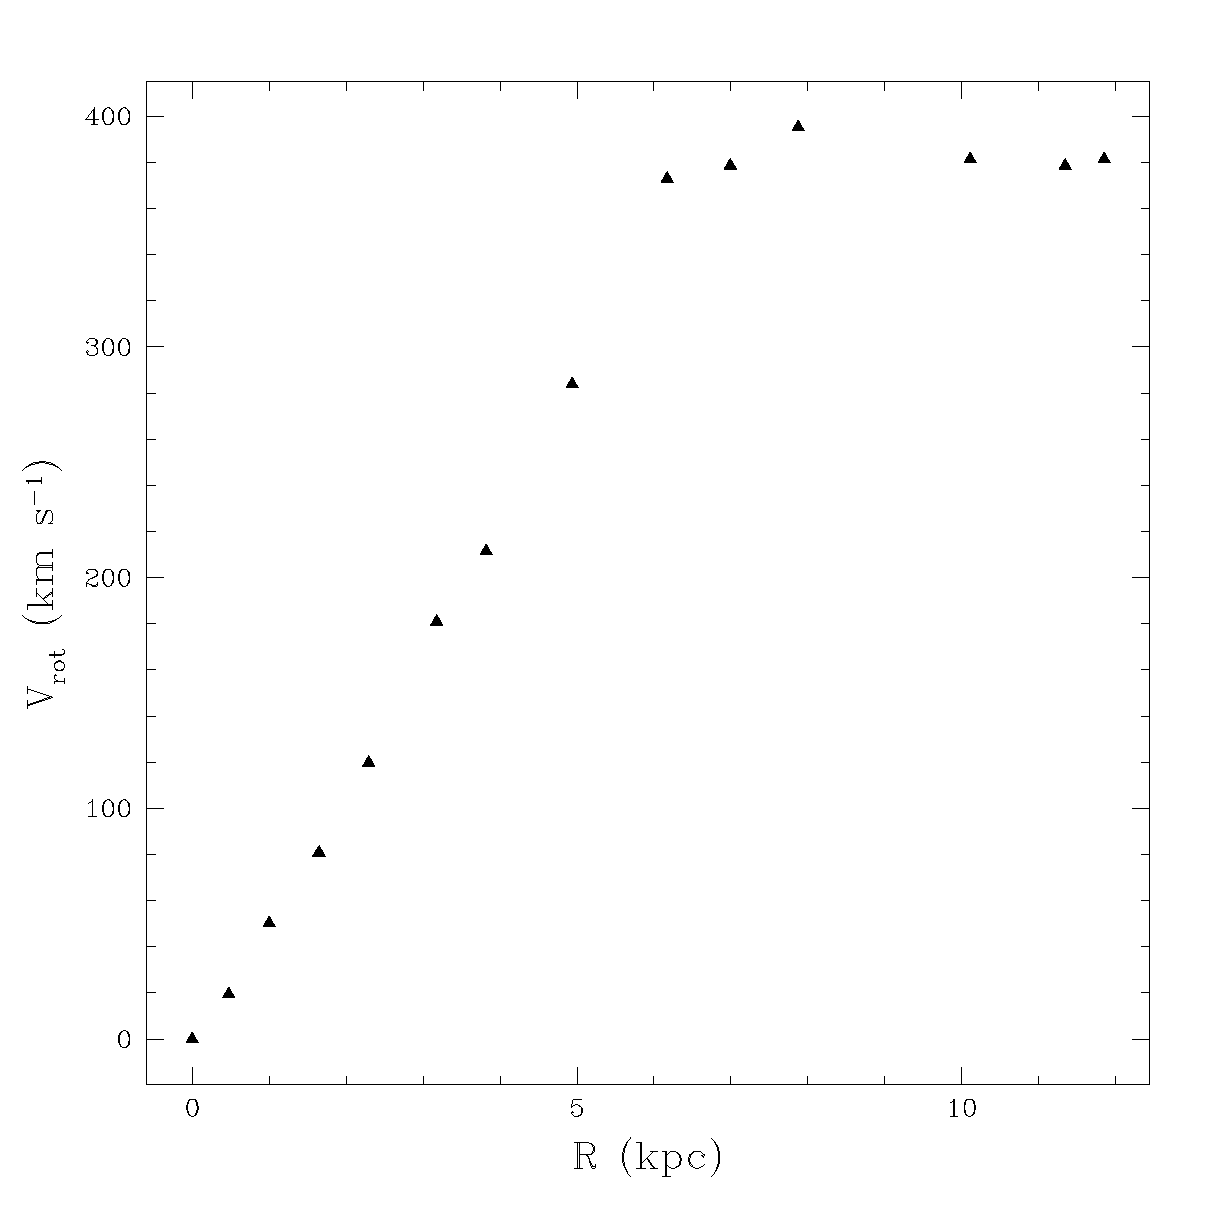
\includegraphics[scale=0.4]{rotcrv.eps}
\caption{Rotation Curve of the Sombrero Galaxy (M104)}
\end{figure}

The rotation curve of M104 exhibits a very fast rise, common of bulge
dominated galaxies. The rotation curve also flattens out around 380
km/s at $\sim$ 6 kpc from the center. 

\section{Discussion}
]
\subsection{Morphology of M104}

\subsection{Mass (Nicolas)}

In order to obtain the mass of the galaxy we assume that the system 
is in equilibrium i.e:
\begin{equation}
2T = U
\end{equation}

This let us compute the velocity terms of the mass of the galaxy, and the radii.

\begin{equation}
mv^{2} = \dfrac{GMm}{r}
\end{equation}

\begin{equation}
v = \sqrt{\dfrac{GM}{r}}
\end{equation}

\end{document}



